%! TeX program = pdflatex
\documentclass{article}
\usepackage[english]{babel}
\usepackage[utf8]{inputenc}
\usepackage{amsmath}
\usepackage{amssymb}
\usepackage{hyperref}
\usepackage{graphicx}
% \usepackage{natbib}
\usepackage{pgf}
% \usepackage{url}
\usepackage{algorithm}% http://ctan.org/pkg/algorithms
\usepackage{algpseudocode}% http://ctan.org/pkg/algorithmicx
% \usepackage{tikz-cd}
\usepackage{listings}
\usepackage{xcolor}
% \usepackage[colorlinks, linkcolor = blue, citecolor = magenta]{hyperref}
\usepackage{tikz}
% % \usepackage{minted}
\usepackage{float}
% \usetikzlibrary{shapes, arrows, positioning}
% \lstset{ 
%     language=Python,                 % the language of the code
%     basicstyle=\ttfamily\small,      % the size of the fonts that are used for the code
%     numbers=left,                    % where to put the line-numbers
%     numberstyle=\tiny\color{gray},   % the style that is used for the line-numbers
%     stepnumber=1,                    % the step between two line-numbers. If it's 1, each line will be numbered
%     numbersep=5pt,                   % how far the line-numbers are from the code
%     backgroundcolor=\color{white},   % choose the background color. You must add \usepackage{color}
%     showspaces=false,                % show spaces adding particular underscores
%     showstringspaces=false,          % underline spaces within strings
%     showtabs=false,                  % show tabs within strings adding particular underscores
%     frame=single,                    % adds a frame around the code
%     rulecolor=\color{black},         % if not rolframe-color may be changed on line-breaks within not black text (e.g. comments (green here))
%     tabsize=4,                       % sets default tabsize to 4 spaces
%     captionpos=b,                    % sets the caption-position to bottom
%     breaklines=true,                 % sets automatic line breaking
%     breakatwhitespace=false,         % sets if automatic breaks should only happen at whitespace
%     title=\lstname,                  % show the filename of files included with \lstinputlisting; also try caption instead of title
%     keywordstyle=\color{blue},       % keyword style
%     commentstyle=\color{green},      % comment style
%     stringstyle=\color{red},         % string literal style
%     escapeinside={\%*}{*)},          % if you want to add LaTeX within your code
%     morekeywords={*,...} 
% }            % if you want to add more keywords to the rol\newenvironment{notation}
\newtheorem{remark}{Remark}
\newtheorem{definition}{Definition}
\newtheorem{property}{Property}

\newcommand{\pder}[2]{\frac{\partial #1}{\partial #2}}

\title{Electrical grid simulation in the COLMENA framework}
\author{Pablo de Juan Vela $^{1}$ \\
        \small $^{1}$eRoots, Barcelona, Spain \\
}
\date{\today}

\usepackage[style=ieee]{biblatex}
\addbibresource{ref.bib}
\setlength{\parskip}{1em} 
\begin{document}
\maketitle

\section{Introduction}
% ANDES intro
COLMENA is a decentralized framework that allows the coordination of multiple agents to solve complex problems. The framework is based on the concept of a colony of agents that can communicate and coordinate to solve a problem. The agents can be programmed to have different roles and behaviors. The objective of the project is to develop a test case for the COLMENA framework in the context of electrical grids using the simulation tools provided by ANDES \cite{grids:models}(later on, potentially others). The resulting goal is to showcase the capabilities of COLMENA in the context of a decentralized electrical grid, providing useful use cases showing noticeable improvements to be derived from this architecture. The present document is an answer to Objective 1 - Development plan for the validation of the platform.




\subsection{Power Grid \& Service definition}
We define an electrical grid as a set of nodes called buses with electrical devices attached to them. The nodes are interconnected between them through branches, traditionally, power lines and/or transformers. The devices connected to each given bus are generators, loads or others types of devices. In ANDES, each device is defined by a set of differential and algebraic equations (DAE) that define how the devices' states change over time.


% \begin{figure}[!htb]
%     \centering
%     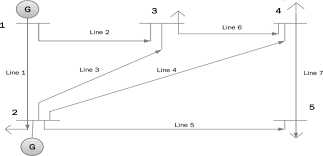
\includegraphics[width=0.7\textwidth]{pictures/5bus.png}
%     \caption{Power grid diagram with buses, lines and generators.}
%     \label{fig:diagram_pairing}
% \end{figure}

\begin{figure}[!htb]
    \centering
    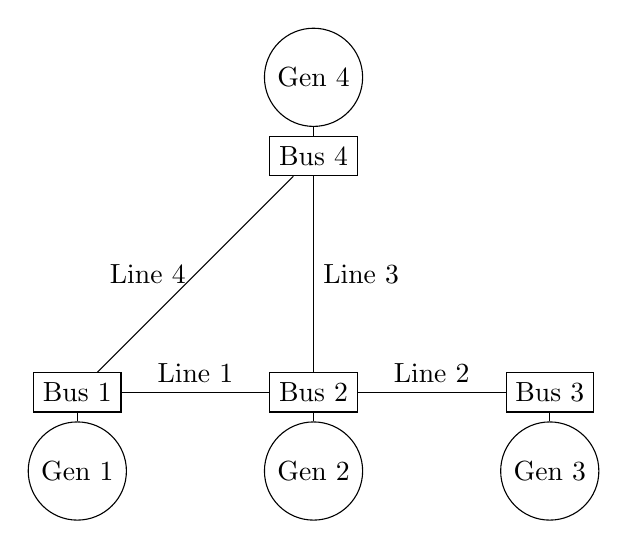
\begin{tikzpicture}
        % Define nodes as rectangles (bars)
        \node[draw, rectangle, minimum width=1cm, minimum height=0.5cm] (A) at (0,0) {Bus 1};
        \node[draw, rectangle, minimum width=1cm, minimum height=0.5cm] (B) at (3,0) {Bus 2};
        \node[draw, rectangle, minimum width=1cm, minimum height=0.5cm] (C) at (6,0) {Bus 3};
        \node[draw, rectangle, minimum width=1cm, minimum height=0.5cm] (D) at (3,3) {Bus 4};
        
        % Define edges
        \draw (A) -- (B) node[midway, above] {Line 1};
        \draw (B) -- (C) node[midway, above] {Line 2};
        \draw (B) -- (D) node[midway, right] {Line 3};
        \draw (D) -- (A) node[midway, left] {Line 4};
        
        % Define generators as circles and connect them to buses
        \node[draw, circle] (G1) at (0,-1) {Gen 1};
        \node[draw, circle] (G2) at (3,-1) {Gen 2};
        \node[draw, circle] (G3) at (6,-1) {Gen 3};
        \node[draw, circle] (G4) at (3,4) {Gen 4};
        
        \draw (G1) -- (A);
        \draw (G2) -- (B);
        \draw (G3) -- (C);
        \draw (G4) -- (D);
    \end{tikzpicture}
    \caption{Simple power grid topology with buses and generators.}
    \label{fig:simple_topology}
\end{figure}

The electrical grid is defined by multiple magnitudes that define its overall state. Some of the more critical metrics that we consider are the following. The one most important to our use case is the frequency since it's linked with most other magnitudes and maintaining the frequency is one of the primary concerns of grid operators.

\begin{itemize}
    \item \textbf{Frequency:} The frequency can be understood as a local measurement that describes the voltage at a specific bus. A device called Phasor Measurement Unit (PMU) can measure the frequency of the bus it is connected to. Maintaining the frequency at the nominal value (e.g. $50$~Hz in Europe) is key for the proper functioning of the grid. Frequency values above or below this value can unbalance the grid from a power point of view or even damage certain components. It is worth mentioning that while the frequency is a local variable, it is often the case that the frequency is the same, or very similar, in all buses.   
    %\item \textcolor{red}{Something to be aware of: is the frequency at each bus a different variable from the synchronous rotor speed? You say the two are very closely related, which is true, but I do not know if ANDES treats them separately.}
    \item \textbf{Synchronous Generator Shaft's Speed}: Synchronous generators are devices that generate power which is then injected to the grid. This is done by magnetically coupling a stator and a rotor that spins at a certain speed, ideally as close as to the nominal frequency. The value of the frequency in the grids buses and the angular speed of the rotor are closely linked and are frequently used interchangeably. In fact, generators can see a drop in their angular speed to mitigate a drop in frequency in a close bus.
    %\item \textcolor{red}{Better to mention voltage magnitude, just to avoid confusion}
    \item \textbf{Voltage Magnitude(V)}: The voltage is a magnitude linked to a specific bus and also needs to be as close to the nominal value as possible. Drops in frequency can be linked to drops in voltage.
    \item \textbf{Power injected/consumed (kW)}: The power injected is by a generator is the amount of power the . The objective of the grid supervisor is to keep the balance of power as close to zero as possible. Raising the amount of power injected by a generator also tends to raise its synchronous speed. It's an important lever in controlling  
\end{itemize}

%\textcolor{red}{From the various available grid measurements, I would emphasize we will focus on the frequency for these first study cases. This will make the following explanation more clear I think.}


\begin{table}[H]
    \centering
    \caption{Summary of the metric's definition.}
    \begin{tabular}{lrr}
        \hline
        \textbf{Magnitude} & \textbf{Unit} & \textbf{Description} \\
        \hline
        \hline
        Voltage & kV & Voltage at a bus \\
        Generator Speed & Hz & Rotations of the shaft per second\\
        Current & A & Current through a branch \\
        Frequency & Hz & Number of voltage sine waves per second\\
        RoCoF & Hz/s & Frequency's derivative \\
        Power Injected & kW & Power injected to the grid by a generator. \\
    \hline
    \end{tabular}
\end{table}
  

The metrics just introduced are key to defining the performance of a grid and to the frequency control response of a power grid. The objective of the frequency response is multiple. On a first time scale (primary response)\cite{source:NRELfrequency}, the control aims to take the system from a transient to a stable condition and avoiding critical values for the frequency. During the secondary response, the objective is to restore the steady state values to their nominal values. Finally, the last response's objective is to restore the the power reserves to their original value \cite{source:bookelectron}.

The objective of the service implemented in COLMENA will be then to aid to the frequency control response by implementing decentralized roles that can improve the performance of the control. These roles will take the form of changing set-points for certain devices, connecting or disconnecting devices such as secondary generators and others. 

Additionally, we will define the different metrics in relations to their context in the grid. This means that every metric is measured in a specific context like a given area or a type of electrical device. This way we can group the values of the previously defined metrics in specific contexts such as the following and develop more specific insights.

\begin{itemize}
\item Local: Measurements that can be done in the same device. 
\item Semi-Local: Measurements that can be done in the devices connected to the same bus. 
\item Regional: Measurements that can be done in the devices from the same given area. 
\item Categorical: Measurements that can be done in the devices of the same type. 
\item Adjacent: Measurements that can be done in the devices that are just one connection away.
\end{itemize}


\subsection{Devices}

Power system simulations, such as the ones performed by the ANDES package, are organized around devices. Each device at a given time $t$ is defined by the value's of the algebraic variables and state variables. Devices of the same type have the same variables. In the context of the frequency service control we have found the following devices that can be useful to the simulation and also present some sort of decentralized control.

%\textcolor{red}{For each device below, explain: its electrical purpose, if they are injections or branches in the topology, and if they can be controlled.}
\begin{itemize}
    \item Synchronous Generators: Traditional sources that convert mechanical energy into electricity to be injected to the grid.
    \item Converters \& distributed generations: Used to convert power from distributed generation from DC to AC, usually associated to some sort of distributed generation.
    \item Loads: They consume power from the grid.
    \item Lines: They connect different buses.
    \item Switches: They allow the flow of power through a Line.
\end{itemize}

In the following sections we will se how these devices fit with the service of controlling the frequency.

\subsubsection*{Synchronous Generators}

Generators are devices that inject power to the grid. A synchronous generator injects electrical power from a rotating part that spins synchronously to the grid's frequency. The synchronous generators in the simulation will be defined by two internal states: $\omega \in \mathbb{R}$ the angular velocity and $\theta  \in \mathbb{R}$ the shaft's angular position. The generator's turbine can set the value of the power being injected by the generator's or the set point for the reference angular speed $\omega_{ref}$. Controlling these set points is key to improve the performance of the grid and impacts the directly on the grid. The generator model used in the simulation can be consulted at \cite{image:diagram:governor} and \cite{source:andes:models:generator}, it also includes the governor's and the exciter's model.

\begin{figure}[!htb]
    \centering
    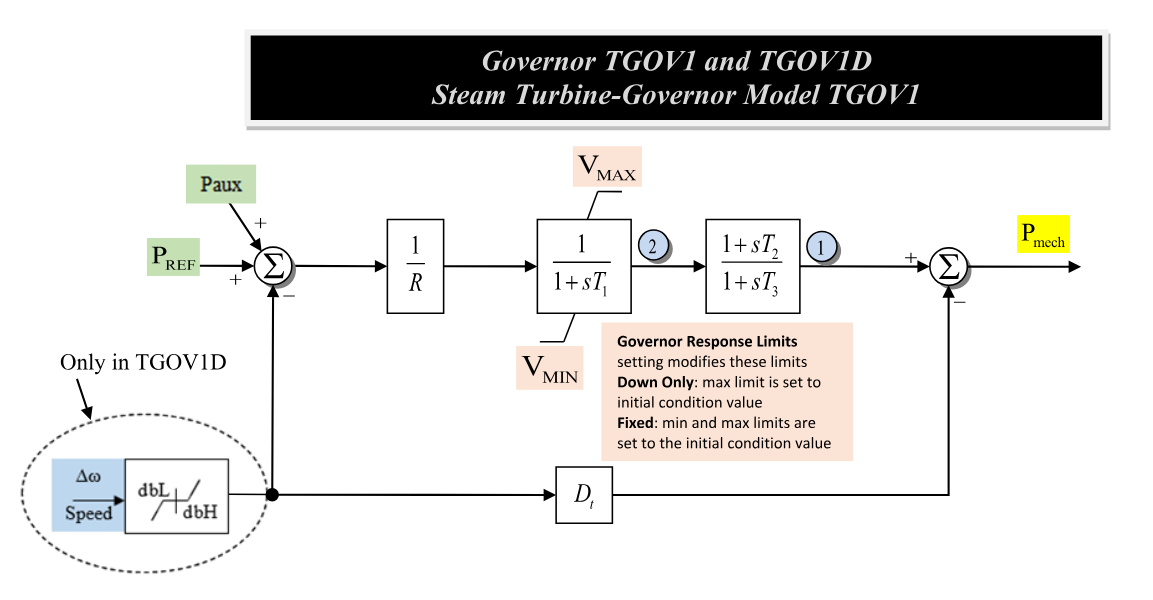
\includegraphics[width=1\textwidth]{pictures/governor.png}
    \caption{Block diagram of a generator's governor controlling the injected power. \cite{image:diagram:governor}}
    \label{pic:governor_diagram}
\end{figure} 

\subsubsection*{Converters \& distributed generation}

Converters can take the form of a Voltage Source Converter (VSC). A VSC is a converter that converts a DC voltage to an AC voltage waveform.  They are commonly used to track the angle of the grid at a bus and inject (or absorb) active and reactive power from an energy source. They are usually paired with DC sources of energy, such as PV plants, as a way to connect them to the grid. We consider a VSC that can operate in two modes: 'Grid following'(GFL) and 'Grid forming'(GFM). 

\begin{itemize}
    \item Grid Following: In the GFL mode, the converter tracks the grid's frequency and injects a controlled power, acting as an ideal current source.
    \item Grid Forming: In the GFM mode, the converter creates its own frequency and imposes a voltage acting as an ideal voltage source.
\end{itemize}

In terms of control, both GFM and GFL have reference values they have to track with controllers. The control is built with the goal of following the reference value as close as possible. For the GFL mode the reference value usually refers to the power injected, while for the GFM its the frequency or voltage. This GFM behavior is quite close to one of a typical synchronous generator. The flexibility and the different set points of this type of converter fit well with the decentralized control principle of COLMENA.

Modelling distributed generation is usually done by combining a DC current source and sometimes a battery that are connected to a AC-DC converter. The converter that is paired to this ensemble can control both the active and reactive power that is injected to the grid and that is stored in the battery (if present). The control of the setup is defined by the parameters $\gamma_p, \gamma_q \in [0,1]$ . These parameters define which proportion of the active and reactive power respectively and generated by the setup is injected to the grid. We can therefore define different set points for the distributed generation depending on the power injected. The power that is not injected is then saved by the battery. This can be expressed as these three different set points:

\begin{itemize}
    \item $\gamma_p = 1$ all of the power generated is injected to the grid.
    \item $\gamma_p = 0$ all of the power generated is stored in the battery.
    \item $\gamma_p = 0.5$ half of the power generated is injected to the grid and half is stored in the battery.
\end{itemize}


\subsubsection*{Loads}

A load is an electrical model that is connected to a bus and consumes a given amount of active and reactive($P$(MW),  $Q $(Mvar) respectively). In the context of the frequency control service, the load device can have varying values of $P$ and $Q$ depending on the state of the grid. More specifically, operators can control the power consumed by enforcing load shedding which consist in reducing part of the power being used. This response can be very useful to the grid in order to adapt to drops in generation or line faults.

\begin{figure}[!htb]
    \centering
    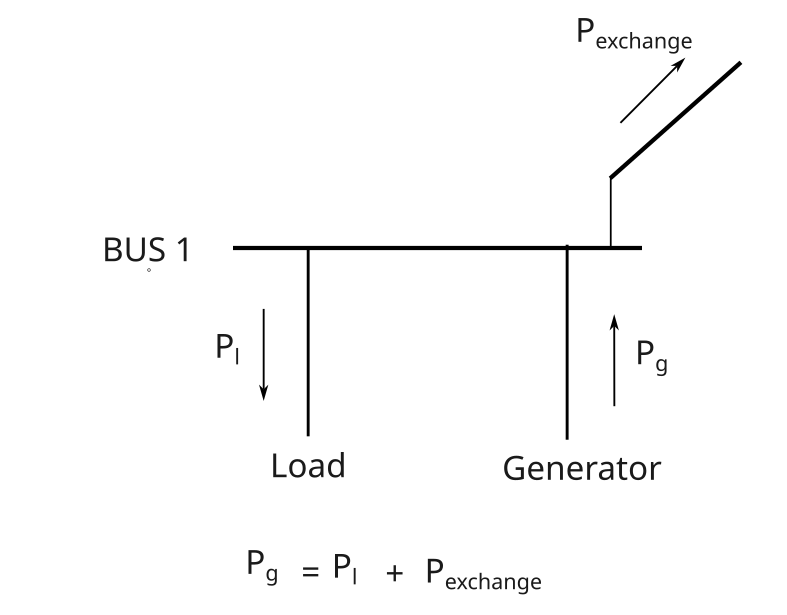
\includegraphics[width=0.5\textwidth]{pictures/busdiagram.png}
    \caption{Bus power exchange diagram.}
    \label{pic:bus_diagram}
\end{figure} 

\subsubsection*{Switches}
Switches are controllable elements that control the connection state of a Line. In this case the set states are just 'Open' or 'Closed'. In the open state no current travels directly between the buses while in the Closed state the line works at normal operation. 

\subsection{Andes-COLMENA Integration requirements}

In this section we explain how ANDES and COLMENA will work during the simulation and how they will communicate. As a standalone, ANDES simulates the time domain response of the power grid for a pre-set amount of time. The package solves the equations numerically and returns the solution but it does not simulate the grid in real time. To enable the integration with COLMENA we modify ANDES into running for a given step-size only when the real time is greater than the simulation time in order for it to catch-up to. ANDES is run parallel to COLMENA on an independent app run on an separate device not part of COLMENA's colony of agents. Specific COLMENA Agents will periodically send requests to the ANDES App to get the simulation's information and to send changes.   

From the COLMENA's side, we will define specific COLMENA-agents that will be paired with a single ANDES-device in the grid. The COLMENA-agent will have two main roles in a continuous manner. They will read their device's variables, store the values internally, and send the behavior changes in the form of new set-point and parameter changes for the paired device. These roles will be the building blocks of the COLMENA-ANDES integration.      

%\textcolor{red}{Here one of the diagrams you had on the slides would be useful}

\begin{figure}[!htb]
    \centering
    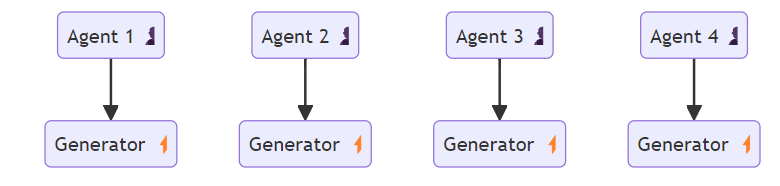
\includegraphics[width=0.7\textwidth]{pictures/colmena_pairing.png}
    \caption{COMENA-Agent pairing diagram.}
    \label{fig:diagram_pairing}
\end{figure}


\section{Use Case Specification}

Having explained the objectives of the project, we want to chose specific scenarios that are well adapted to evaluate these objectives. In this particular case, we are looking for power grids of considerable size, and with the appropriate types of devices presented earlier such as generators and converters to facilitate the integration of distributed generators. Additionally, we would want to choose use cases in which the grid can be separated into different areas to properly implement different geographical contexts to take into account. Finally, we also consider the ease to access information and data about the modeled grid. We consider the following as interesting candidates: 

\begin{itemize}
    \item Kundur 2-area system \cite{grids:kundur}
    \item IEEE-118 bus test case \cite{grids:ieee118} 
    \item IEEE 300 bus test case  \cite{grids:ieee300} 
    \item ACTIVSg 2000 bus test case  \cite{grids:activsg2000} 
\end{itemize}


For the first use case we propose first using the grid defined in the Kundur two area system  \cite{grids:kundur}. This grid consists of 10 buses divided in 2 areas. Each area includes two synchronous generators. Additionally, this simulation includes a line failure at a specific time step (Line 8, at $t=2$~s). The objective of this is to showcase how the decentralized nature of COLMENA can adapt to unexpected events in the grid such as failures and avoid cascading failures in the grid. 

\begin{figure}[!htb]
    \centering
    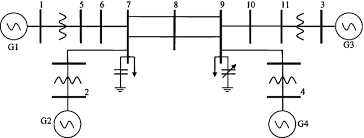
\includegraphics[width=0.7\textwidth]{pictures/kundurgrid.png}
    \caption{Kundur grid scheme. \cite{grids:kundur}}
    \label{fig:kundur2}
\end{figure}

In this specific use case the COLMENA-Agent will be paired with a generator   and monitor the values provided by the ANDES simulation. Moreover, this agent will be able to modify some of the generators values such as the power injected or internal controlling parameters. The objective is to overtime include different sources of generation and the proposed GFL-GFM converters. Let's see a proof of concept of what the integration could look like. In this use case one of the COLMENA Agents is able to modify the inertia parameter of the generator 1 inside the simulation depending of the value of the generator's speed $\omega$. By modifying the inertia parameter $M$ we expect to see is the generator's angular velocity $\omega$ having 2 distinct behaviors.  

\begin{table}[H]
    \centering
    \begin{tabular}{|l|l|l|}
    \hline
    Operating State & KPI                              & Parameter $M$ value \\ \hline
    A               & $\omega \in [1 - \varepsilon, 1 + \varepsilon]$ & 12  \\ \hline
    B               & $\omega \notin [1 - \varepsilon, 1 + \varepsilon]$ & 120               \\ \hline
    \end{tabular}
    \caption{Generator set-points summary.}
\end{table}
  

\begin{figure}[h]  % [h] places the figure "here"
    \centering
    % Fit the PGF figure to the page width
    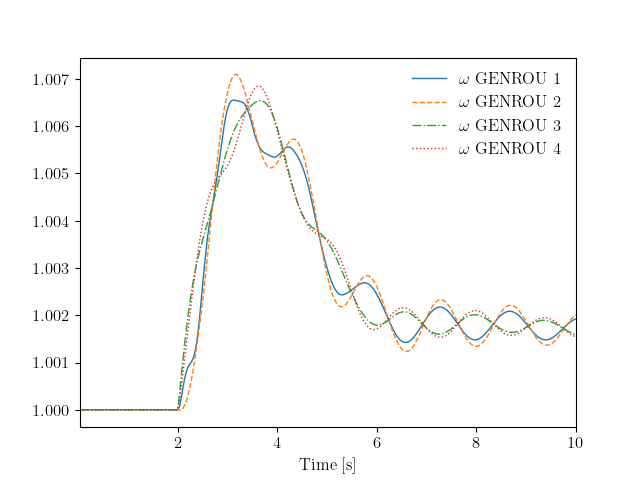
\includegraphics[width=1\textwidth]{pictures/plot.png}

    \caption{Time series of the distributed generator's frequency.}
    \label{fig:sample_figure2}
\end{figure}

Once this more accessible use case is deployed, our next goal is to scale the simulation to a more extensive grid that could be able to showcase the performance of COLMENA in a more complicated environment, with more varieties of models and more complicated controls overall. The objective is to eventually run the simulation in larger grids with a larger number of agents. For this we can use other test grids such as the IEEE 118 bus case \cite{grids:ieee118}. This test grid is composed by 118 buses, 54 generators and 99 Loads. Additionally, some of the generators are synchronous condensers which are essentially synchronous motors whose shaft is not connected to any mechanical load. Their main function is to provide reactive power compensation. Moreover, it uses the same models as the ones used in the previous tests cases so transferring the already developed models is feasible.

\begin{figure}[h!]
    \centering
    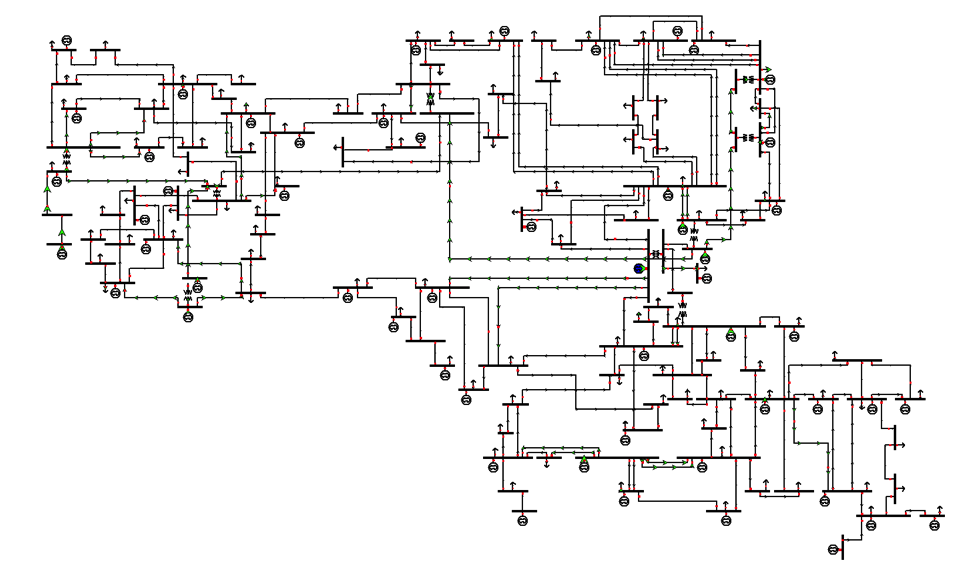
\includegraphics[width=1\textwidth]{pictures/IEEE118.png}
    \caption{IEEE118 grid scheme. \cite{grids:ieee118}}
    \label{fig:kundur}
\end{figure}

\subsection{Grid's Performance \& Key Performance Indicators}

In the first section we have defined a set of metrics and states that are key to defining the grids state, specifically when dealing with the frequency response. These include the frequency, the angular speed of the synchronous generators and others. We aim to define key performance indicators (KPI) starting from the metrics defined previously. These KPIs define the performance of the grid with respect to the frequency service control. 

\begin{itemize}
    \item Minimum and maximum of the generator's frequency.
    \item Minimum and maximum of the mean bus frequency in an area from the nominal frequency.
    \item Voltage steady state values.
    \item Rate of Change of Frequency (RoCoF).
    \item Available power reserves.
    \item Power Balance \& regional power exchanges.
    \item N-1 criteria
    \item Power Losses
\end{itemize}

%\textcolor{red}{A few questions. What do you mean by steady-state values? (I mean, which magnitude? Voltages, currents...?) Also, the $N-1$ criteria will be very hard to assess I believe. Same applies to the economic criteria as we have no information on costs for these grids. Some ideas to add: percentual power losses, maximum overloading of lines, short-circuit currents.} 

\subsection*{Minimum and maximum of the generator's frequency}

This KPIs is usually used with regards to the primary response in the frequency control response. The objective would be to maintain the generator's frequency $\omega$ as close to the nominal value. In moderately strong power grids a common value for this KPI would be around $0.1\%$ around the nominal value. This is true for both the generator's frequency and the buses' frequency.

\subsection*{RoCoF}

The Rate of Change of Frequency is the frequency's time derivative measured in a given bus. It signals sudden changes in frequency and if its close to $0$ for a given amount of time it can also signal the grid reaching a steady state. Therefore the RoCoF is key to measure the performance of the grid during transients. 

\subsection*{Available Power Reserves}

The available power reserves is the amount of power that can be activated in a given amount of time in case of need but its not being used. It usually considers an horizon of 10 to 30 minutes. Additionally, we also need to consider the ramp up and ramp down capabilities of these power reserves. The ramp up measured in kW/s and is the speed with which this reserve power can come online. These power reserves come in the form of battery storage and ancillary generators that can be ramped up when necessary. Similarly, ramp down The grid operator usually defines minimum requirements for available power values.


\subsection*{Maximum line current}

The current through a line is limited by a maximum value for security purposes. If the current through a line surpasses the maximum value for a specific amount of time the line can disconnect to avoid being damaged.

\subsection*{Regional monitoring \& power exchanges}

Regional power imbalances can occur within interconnected grids.
To monitor and manage these regional imbalances, a key indicator is the Area Control Error (ACE). The ACE of a region is defined as the difference between the scheduled power exchange and the actual power exchanged neighboring regions. A well-performing grid aims to keep the ACE values of all regions close to zero, indicating that actual power flows are aligned with the planned schedules. Excessive reliance on interconnections to balance regional loads can compromise grid security and resilience. Furthermore, imbalances in one region can propagate to neighboring regions through interconnections, potentially leading to cascading failures and widespread blackouts. Therefore, it's essential to monitor the power exchanges between regions.

\subsection*{N-1 criteria}

The N-1 criterion is a standard used in power system planning and operation to ensure reliability and resilience. It specifies that a power system should be able to withstand the loss of any single element (like a generator, transformer, or transmission line) without causing a system-wide failure. New devices could be connected or scheduled by the COLMENA agents to help ensure the criterion is respected. 

\subsection*{Power Losses}

Grid performance is also influenced by power losses and reactive compensation. Power losses, primarily due to resistance in transmission lines, reduce overall efficiency and increase operational costs. To mitigate these losses, reactive compensation is used, which balances reactive power in the grid, improving voltage stability and reducing strain on transmission infrastructure. 

\subsection{Role Definitions}

The envisioned integration of Andes and COLMENA places a special focus on the grid's frequency control response. For this purpose we propose a set of roles that can be taken by the COLMENA agents in order to control the grid in a decentralized grid. The roles are explained descriptively.  

\subsubsection*{Device Basic Role}

The device basic role defines the basic operations needed for the agents and devices to coordinate through Andes-COLMENA. The agent that takes on this role is supposed to be paired to a single device of type generator, although we can consider this role being taken multiple times by the same agent in order to control multiple devices. In this case the device basic roles is persistent and has the following functions:

 \begin{itemize}
     \item Initializes a client that calls Andes and sets up the exchange of information.
     \item Stores the state and algebraic variables relative to the device it is paired up.
     \item Changes the parameter when it receives the message to do so through the appropriate channel.
     \item Changes the behavior of the device when instructed to do so through the appropriate channel.
 \end{itemize}

Taking the example of a generator device this role has the requirement of having a generator and at least these 2 channels:

\begin{itemize}
    \item Channel Generator parameter change: where it receives both the parameter to change and the new value.
    \item Channel Generator measurements: where it publishes the frequency of the generator every time step.
\end{itemize}

\subsubsection*{Rotor Speed Optimizer}

This role is specific to agents with the "generator" requirement. It is activated when the rotor's speed exhibits unusual behavior, such as high values or high Rate of Change of Frequency (RoCoF). This role defines the optimal reference value for the rotor's speed, $\omega_{ref}$to facilitate frequency control during transient states. One objective of this role is to avoid excessive oscillation in the frequency and getting to a steady state during the primary response.

The role can be subdivided into transient and steady-state modes, as its behavior may differ depending on the grid's overall state.  

\subsubsection*{Rotor Speed Setter}

This role, specific to agents with the "generator" requirement, receives a reference rotor speed $\omega_{ref}$ and modifies the generator's parameters to achieve this target value. The set of actions performed are actions are:

\begin{itemize}
    \item Reading the $\omega_{ref}$ continuously.
    \item Adapt the control strategy in Andes through a parameter change.
    \item Deactivate the role when the $\omega \in [\omega_{ref} - \varepsilon, \omega_{ref} + \varepsilon]$ in the steady state.
\end{itemize}

This role will usually adapt the generator's power in order to get the desired speed. More generally, we can imagine this role being extended to set other types of variables in a given device. This could be implemented through a feedback control loop or through a feed forward control loop. These are strategies that can be represented as a block diagram where the input signal is the difference between a reference value and the real value. 

\subsubsection*{Voltage Optimizer Role}

This role, specific to COLMENA agents paired with electrical devices and capable of control, computes the optimal voltage when deviations occur from the desired voltage set point, considering multiple objectives such as minimizing power losses, maximizing voltage stability, and ensuring system security.

For example, the role would:

\begin{itemize}
    \item Prioritize voltage stability: If the system is experiencing voltage fluctuations, the role may prioritize actions that stabilize the voltage, even if it means slightly increasing power losses.
    \item Optimize power losses: During periods of high demand, the role might focus on minimizing power losses by adjusting the voltage to reduce resistive losses in transmission lines.
\end{itemize}

The specific optimization techniques used will depend on the capabilities of the agent and the specific requirements of the grid.
\subsubsection*{Load Shedding Role}

This role can be taken by agents associated with a load consuming device in the grid. It is activated in the secondary response to counter a drop in frequency.

\begin{itemize}
    \item Continuously diminishes the power being used by the load.
    \item When the frequency is back to a nominal value, it goes back to the desired power.
\end{itemize}

\subsubsection*{Reserve Activation Role}

This role can be taken by agents associated with ancillary generation or batteries consuming device in the grid. It is activated in the secondary response to counter a drop in frequency.

\begin{itemize}
    \item Connect or Disconnect the reserve to the grid.
    \item Set the power injected to the grid.
\end{itemize}

\subsubsection*{Area Monitoring Role}

This role can be taken by agents associated with in a specific geographical area. The role monitors the power balance of that area with the rest of the grid. It has access to the appropriate communication channels. When activated it's charged with:
\begin{itemize}
    \item Monitoring the power balance in the area. 
    \item Flagging failure in the scheduling of the power exchanges.
    \item Isolate problematic regions that could provoke a cascading failure.
\end{itemize}

\subsubsection*{Current Security role}
If the intensity's value through the line is above the security current then publish the change of behavior in the appropriate channel. It also disconnects line to avoid a cascading failure in the grid. This role could be expanded to take into account other types of failure that damage the grid such as short-circuited lines and gives appropriate adaptations to the grid. Finally, it tries to reconnect the faulted line by adapting the voltage at each end bus
and reconnect the grid if possible.


\section{Current Work}

The current state of the work can be accessed in the Github \href{https://github.com/eRoots-Analytics/COLMENA}{following repository}. The current work can be separated into three main parts:

\begin{itemize}
    \item A modified version of Andes Curent to be run in parallel to the service application.
    \item The testing of different device's behaviors that can be then implemented as roles.
    \item The implementation of the Frequency Control Service using the colmena package.
\end{itemize}

\subsection{Modified Andes}

The original Andes 

\subsection{Frequency Service Deployment}


\section{Conclusion \& Future work}

Grid performance through decentralized control strategies presents an interesting opportunity for the COLMENA framework. By pairing agents with grid components, such as generators and converters, COLMENA could enable real-time monitoring and control adjustments that enhance grid stability, particularly in response to frequency disturbances and power imbalances. This approach was explored using the Kundur test case to showcase the potential of COLMENA. COLMENA could change the behavior of agents in response to changes in KPIs such as frequency stability. The agents would then send messages through the appropriate channels signaling changes in the set point of the devices that would be reflected in the ANDES simulation.

Future work should focus on expanding the scope and complexity of the use cases. This includes integrating a broader range of devices, such as advanced energy storage systems, and simulating additional scenarios that include renewable energy sources and demand response mechanisms. More specifically, we want to deploy a use case in the IEEE 118 bus system. Additionally, we will focus on clearly defining the communication channels between COLMENA agents, and the contexts  and requirements that define the agents in the COLMENA framework for this use case. Finally, we also want to develop and implement more complex roles that could control multiple devices at a time in a specific area and coordinate the response between different areas.  


\nocite{*}
\printbibliography
\end{document}
